%%%%%%%%%%%%%%%%%%%%
%                 File Experiment00.tex        %
%                 Experiment M-0               %
%                   Introductory lab           %
%                                              %
%%%%%%%%%%%%%%%%%%%%

\labChapter{I}{Introductory Lab: Domino Size \& Density}
\label{lab:Intro}
% Introduction
%\section{Introduction}
\section{Background}

\subsection{Measurements}

Physical measurements are more than a simple numerical value. They are specified by:
\begin{enumerate}
\item[$\triangleright$] A physical dimension which is a product of powers of base physical dimensions such as length, time, and mass. Other dimensions include, for example, electric charge. 

\item[$\triangleright$] A choice of units. Usually we use SI units: meter \((\metre)\), second \((\second)\), and kilogram  \((\kilogram)\). 

\item[$\triangleright$] A numerical value that depends on the choice of units.

\item[$\triangleright$] A range of the numerical value depending on the accuracy of measurements. 
\end{enumerate}
Calculations performed using physical quantities follow certain rules: 
\begin{enumerate}

\item[$\triangleright$] Scalar physical quantities can be added or subtracted only if they have the same units. 
\item[$\triangleright$] Scalars can be multiplied (or divided). The same action must be performed on the values and on the units.

\end{enumerate}


Volume $V$ and mass $m$ are two measures of the size of an object. If an object is made of a uniform material, then doubling the amount of material will double both its mass and its volume.  
Density $\rho$ is ratio of mass to volume. 
\begin{equation} \label{eq:I01}
	\rho=\frac{m}{V}.
\end{equation}
Density is a material property, independent of the amount of material or shape of the object. 
The volume of a rectangular parallelepiped shape, i.e., a box, is the product length times width times height \(V=l\cdot w\cdot h\).


\subsection{Estimating Error}
The accuracy of a measurement depends on the limits of the instrument, and on skill in using the instrument.
One estimate of the accuracy of a measurement is to independently repeat the measurement multiple times and observe the \textbf{range and standard deviation of the results}. Another approach is to determine the \textbf{instrument tolerance or precision}.  

Measurement errors change calculated or derived results in different ways, depending on how the quantities enter equations. 
For example, if the measured mass is larger than the actual mass, then the calculated density will also be larger. 
Suppose, on-the-other-hand, that the measured volume is larger than the actual volume.  Because the volume appears in the denominator of Eqn.~\ref{eq:I01}, the calculated density will be reduced. 


\section{Experimental Procedure}

\begin{figure}[h]
  \begin{center}
    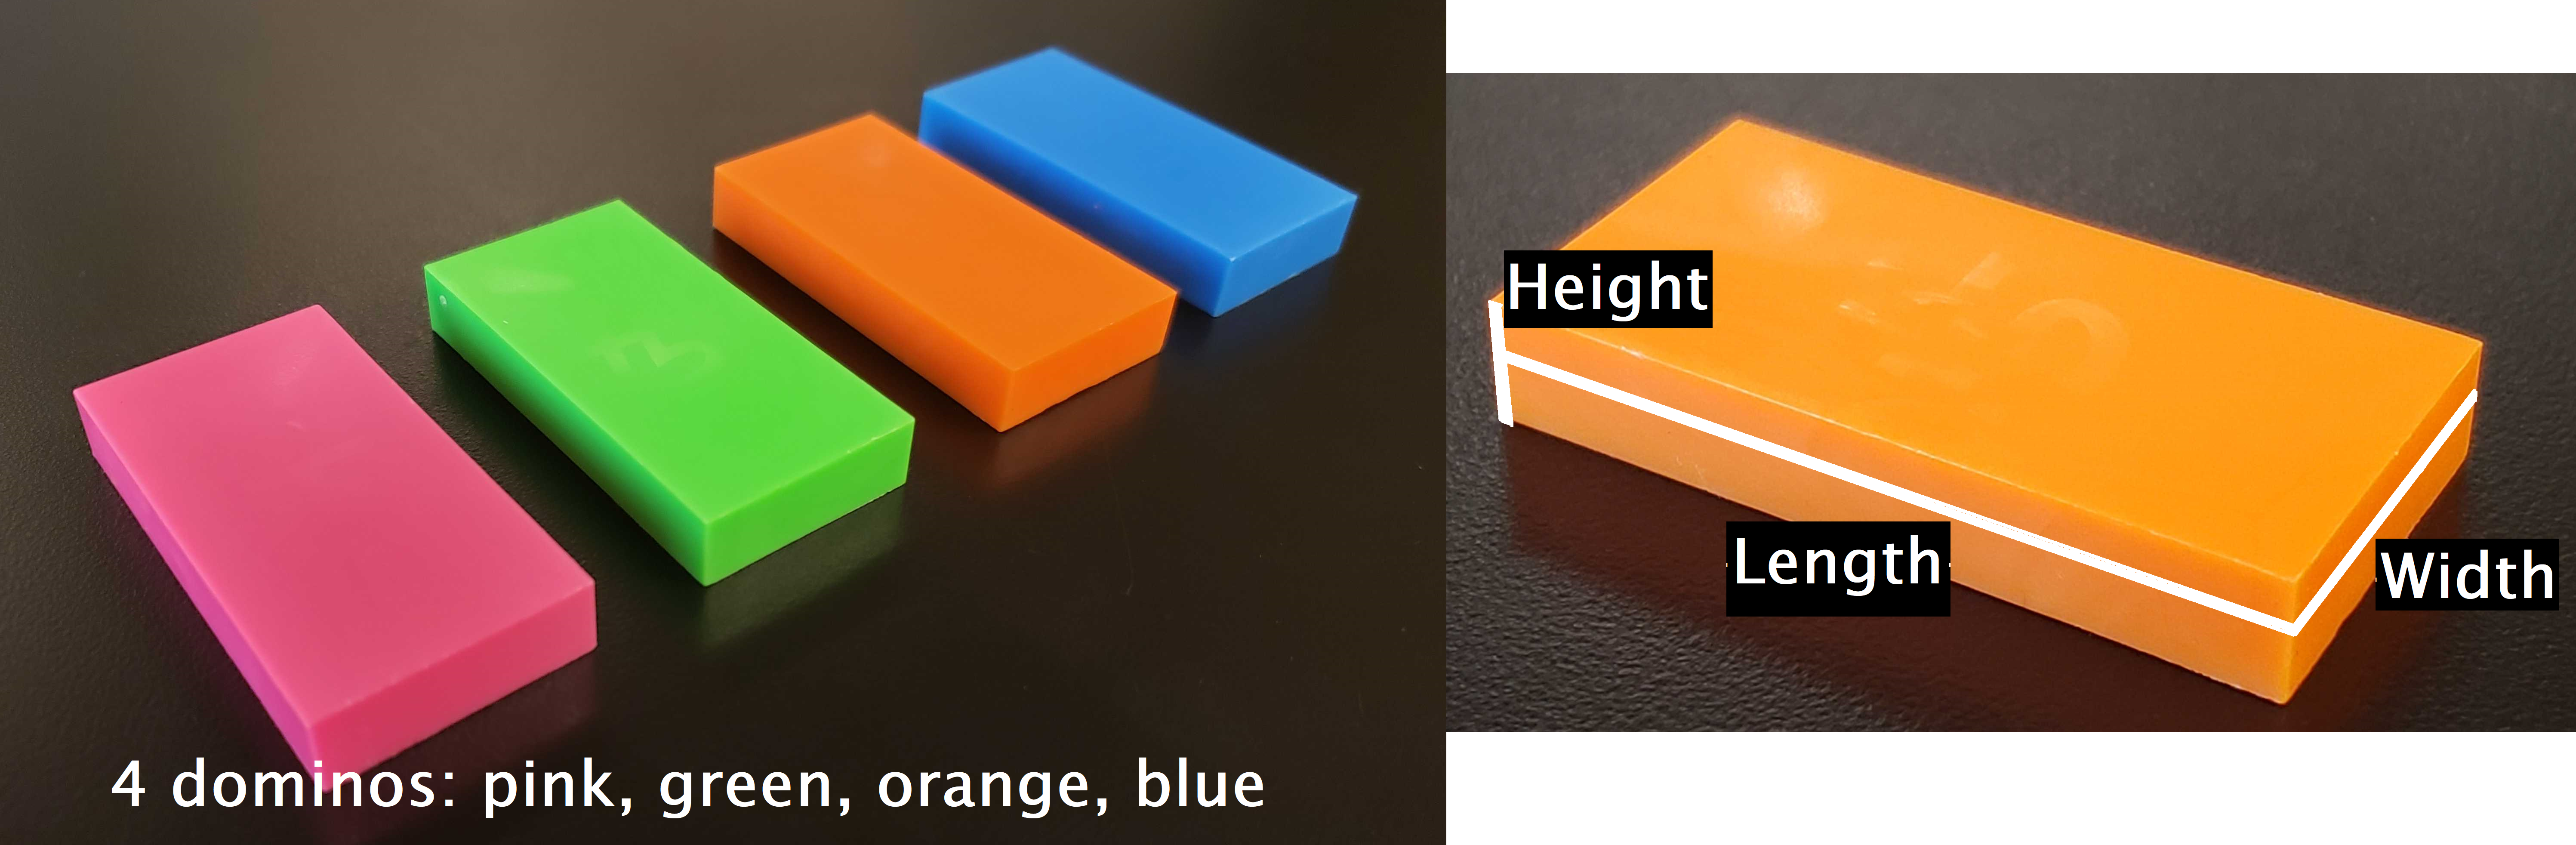
\includegraphics[width=4.9in]{Fall/Experiment00Figures/M0_dominos.png}
  \end{center}
  \caption{Left) Dominoes provided. Right) Relevant length, width, height dimensions of the dominoes.}
  \label{M00Fig01}
\end{figure}

\begin{enumerate}

\item \textbf{OVERALL GOALS:} 
\begin{itemize}
    \item[$\triangleright$] Understand how to take length and mass measurements.
    \item[$\triangleright$] Understand how to characterize measurement uncertainties with standard deviation.
    \item[$\triangleright$] Understand how to characterize measurement uncertainties due to instrument precision.
    \item[$\triangleright$] Each member of the lab group will independently measure the mass, length, width, and height of four provided dominoes per group (i.e. each group gets a pink, green, orange, and blue domino).
\end{itemize}

\textit{NOTE:} It is good practice to \textbf{complete the analysis of trials as you do the experiment}. If there is some error in your experimental method or in your calculation, you can correct it before completing all the other trials. The formulas of the rows for later trials can be created by copying the first trial.

The density of the dominoes' plastic and water are roughly the same. Estimate the value you expect in SI units ($\kilogram/\meter^{3}$). 

\begin{itemize}
	\item[$\triangleright$] Create a Common Data Table for values used in all the trials. In this case, include the instrumental tolerance of the lab scale and the Vernier caliper. 
	\item[$\triangleright$] Create a row for each domino trial. A trial is the measurement by one lab group member of one domino color.
	\item[$\triangleright$] Create a Data Table with columns for:
		\begin{itemize}
			\item Initials of the experimenter
			\item Color of the domino
			\item Measured length $l$, width $w$, height $h$ measured with Vernier calipers and mass $m$ measured with the triple-beam balance in the instruments' units (e.g. mm, $\gram$, etc.)
            \item $l$, $w$, $h$, and $m$ converted to SI units
			\item Calculated volume $V_\text{color}$ for the trial in SI units
			\item Calculated density $\rho_\text{color}$ for the trial in SI units
		\end{itemize}
\end{itemize}

Create a Data Analysis table including:  
\begin{itemize}
    \item Analysis Table 1:
    \begin{itemize}
    	\item[$\triangleright$] Average and standard deviation of the $l_\text{avg.}$length, width, height, volume, and density of each color of domino. 
	   \item[$\triangleright$] Maximum and minimum values of the density and volume based on your experimental value and the instrumental tolerance (i.e. $\pm$ values). \textbf{NOTE:} To maximize Volume $V$, maximize $l$, $w$, $h$. To maximize density $\rho$, maximize $V$ and minimize $m$.
    \end{itemize}
    \item Analysis Table 2:
    \begin{itemize}
        \item[$\triangleright$] Average of the length, width, height, volume, and density of the color set measured by each lab group member.  
    \end{itemize}
\end{itemize}

\end{enumerate}

\pagebreak

\section{Post-Lab Submission --- Interpretation of Results}

\begin{itemize}
    \item[$\triangleright$] Make sure to submit your finalized data table (Excel sheet).
	\item[$\triangleright$] Discuss: Are the densities of all the different colored dominoes the same (within experimental uncertainty based on measurement uncertainties)? Example, do all the $\rho_{\text{blue-person1}}$, $\rho_{\text{blue-person2}}$, etc. agree?
	\item[$\triangleright$] Discuss: Are the average densities of all four dominoes as measured by each person consistent (within experimental uncertainty based on measurement uncertainties)? Example, do all the $\rho_{\text{blue-person1}}$, $\rho_{\text{green-person1}}$, etc. agree?
	\item[$\triangleright$] Discuss: Do you expect the dominoes to float in water (at room temperature)?
    \item[$\triangleright$] What was the precision of your equipment (calipers, triple-beam balance, etc.)?
    \item[$\triangleright$] What are possible systematic errors of the experiment?
\end{itemize}

